% ─────────────────────────────────────────────────────────────────────────
%  CVPR 2026  ·  Learning Eigenstructures of Unstructured Data Manifolds
%  Conference poster  ·  213 cm × 107 cm  ·  4-column landscape
%
%  Compile with LuaLaTeX (preferred) or XeLaTeX so Libertinus loads:
%      lualatex poster.tex
%      lualatex poster.tex       % run twice for refs
% ─────────────────────────────────────────────────────────────────────────
\documentclass[final,t]{beamer}

% ─── Poster geometry ────────────────────────────────────────────────────
% beamerposter wants the size in CM; orientation=landscape is implicit
% when width > height.  scale=1.0 means 1 cm in the PDF == 1 cm physical.
\usepackage[size=custom, width=213, height=107, scale=1.0]{beamerposter}

% ─── Fonts (Libertinus, matches the deck) ───────────────────────────────
\usepackage{fontspec}
\setmainfont{Libertinus Serif}
\setsansfont{Libertinus Sans}
\setmonofont{Libertinus Mono}
\usepackage{unicode-math}
\setmathfont{Libertinus Math}

% ─── Math, graphics, layout ─────────────────────────────────────────────
\usepackage{amsmath, amssymb}
\usepackage{graphicx}
\usepackage{caption}
\usepackage{tikz}
\usetikzlibrary{calc, positioning, arrows.meta}
\usepackage{xcolor}
\usepackage{ragged2e}
\usepackage{array}
\usepackage{booktabs}
\usepackage{enumitem}
\setlist{nosep, leftmargin=*, topsep=4pt, partopsep=0pt}
\usepackage[normalem]{ulem}

% ─── Palette (mirrors the Slidev deck's style.css) ──────────────────────
\definecolor{cFg}        {HTML}{0F172A} % slate-900 — primary text
\definecolor{cFgBody}    {HTML}{1F2937} % slate-800 — body
\definecolor{cFgMuted}   {HTML}{475569} % slate-600 — secondary
\definecolor{cFgSubtle}  {HTML}{94A3B8} % slate-400 — labels
\definecolor{cBgSoft}    {HTML}{F8FAFC} % slate-50  — card bg
\definecolor{cBorder}    {HTML}{E2E8F0} % slate-200
\definecolor{cBrandFrom} {HTML}{4E4376} % deep indigo
\definecolor{cBrandTo}   {HTML}{2B5876} % deep teal-blue
\definecolor{cAccent}    {HTML}{B45309} % amber-700
\definecolor{cDanger}    {HTML}{B91C1C} % red-700

% ─── Beamer theme overrides ─────────────────────────────────────────────
\usetheme{default}
\setbeamercolor{background canvas}{bg=white}
\setbeamercolor{normal text}{fg=cFgBody}
\setbeamerfont{normal text}{size=\normalsize}
\setbeamertemplate{navigation symbols}{}
\setbeamertemplate{itemize item}{\color{cBrandFrom}$\bullet$}
\setbeamertemplate{itemize subitem}{\color{cBrandFrom}\textendash}

% Block (section card) styling
\setbeamercolor{block title}{fg=white, bg=cBrandFrom}
\setbeamercolor{block body} {fg=cFgBody, bg=cBgSoft}
\setbeamerfont{block title}{family=\sffamily, series=\bfseries, size=\large}
\setbeamertemplate{block begin}{
  \begin{beamercolorbox}[wd=\textwidth, ht=2.4ex, dp=1.2ex, leftskip=1ex, rightskip=1ex]{block title}
    \insertblocktitle
  \end{beamercolorbox}
  \begin{beamercolorbox}[wd=\textwidth, leftskip=1ex, rightskip=1ex, vmode]{block body}
    \vspace{0.25ex}
    \justifying
}
\setbeamertemplate{block end}{
    \vspace{0.5ex}
  \end{beamercolorbox}
  \vspace{0.9ex}
}

% ─── Title block (big banner across the top) ────────────────────────────
\title{\textbf{Learning Eigenstructures of Unstructured Data Manifolds}}
\author{%
  Roy Velich$^{1}$ \quad Arkadi Piven$^{1}$ \quad David Bensa\"id$^{1}$ \quad
  Daniel Cremers$^{2}$ \quad Thomas Dag\`es$^{1}$ \quad Ron Kimmel$^{1}$%
}
\institute{$^{1}$\,Technion --- Israel Institute of Technology \quad
           $^{2}$\,Technical University of Munich}

% ─── Header band ────────────────────────────────────────────────────────
\setbeamertemplate{headline}{%
  \begin{beamercolorbox}[wd=\paperwidth, ht=12cm, dp=0pt, leftskip=2cm, rightskip=2cm]{background canvas}
    \vspace{1.4cm}
    \centering
    {\color{cFg}\fontsize{96pt}{110pt}\selectfont\bfseries \inserttitle\par}
    \vspace{0.6cm}
    {\color{cFgMuted}\fontsize{40pt}{52pt}\selectfont \insertauthor\par}
    \vspace{0.35cm}
    {\color{cFgSubtle}\fontsize{32pt}{42pt}\selectfont \insertinstitute\par}
    \vspace{0.3cm}
    \rule{0.6\paperwidth}{1.5pt}\par
    \vspace{0.2cm}
    {\color{cBrandFrom}\fontsize{34pt}{42pt}\selectfont\bfseries CVPR 2026 \;·\; Oral Presentation\par}
  \end{beamercolorbox}
}
\setbeamertemplate{footline}{}

% ─── Column width helpers (4-col layout with 1 cm gutters) ──────────────
%  Total width = 213 cm.  Side margins ≈ 1.5 cm each.
%  Working width = 210 cm.  Three gutters of 1.5 cm each (4.5 cm total).
%  Per-column width = (210 - 4.5) / 4 = 51.375 cm  ≈  0.2417 \paperwidth
\newlength{\colwidthA}\setlength{\colwidthA}{51.4cm}

\begin{document}
\begin{frame}[t]

% ─────────────────────────────────────────────────────────────────────────
%  COLUMN BAND  (sits below the header band rendered by \setbeamertemplate)
% ─────────────────────────────────────────────────────────────────────────
\vspace{0.4cm}
\begin{columns}[t, onlytextwidth]

% ───────────── Column 1 ─────────────
\begin{column}{\colwidthA}

\begin{block}{Motivation}
  Spectral methods on manifolds underpin shape correspondence, descriptors,
  manifold learning, ARAP, and many more downstream tools.
  But computing the Laplacian eigenstructure on raw, unstructured point
  clouds is delicate: it requires explicit mesh/graph construction,
  cotangent or heat-kernel weights, then a numerical eigensolve --- and
  none of it is differentiable.
  \vspace{0.4ex}

  \textbf{Goal.}\; Learn an ordered eigenbasis of the manifold's
  Laplace--Beltrami operator (LBO) \emph{directly} from a point sample,
  bypassing the discretization pipeline.
\end{block}

\begin{block}{The Laplacian, in one slide}
  % Row 1 — same minipage height so both titles sit on the same top line;
  % the shorter data-manifold composite is centred vertically inside its cell.
  \newlength{\toprowH}\setlength{\toprowH}{14.5cm}
  \begin{minipage}[t][\toprowH][t]{0.48\linewidth}
    \centering
    {\small\textbf{On a data manifold}}\par
    \vspace{0.4ex}
    \vspace*{\fill}
    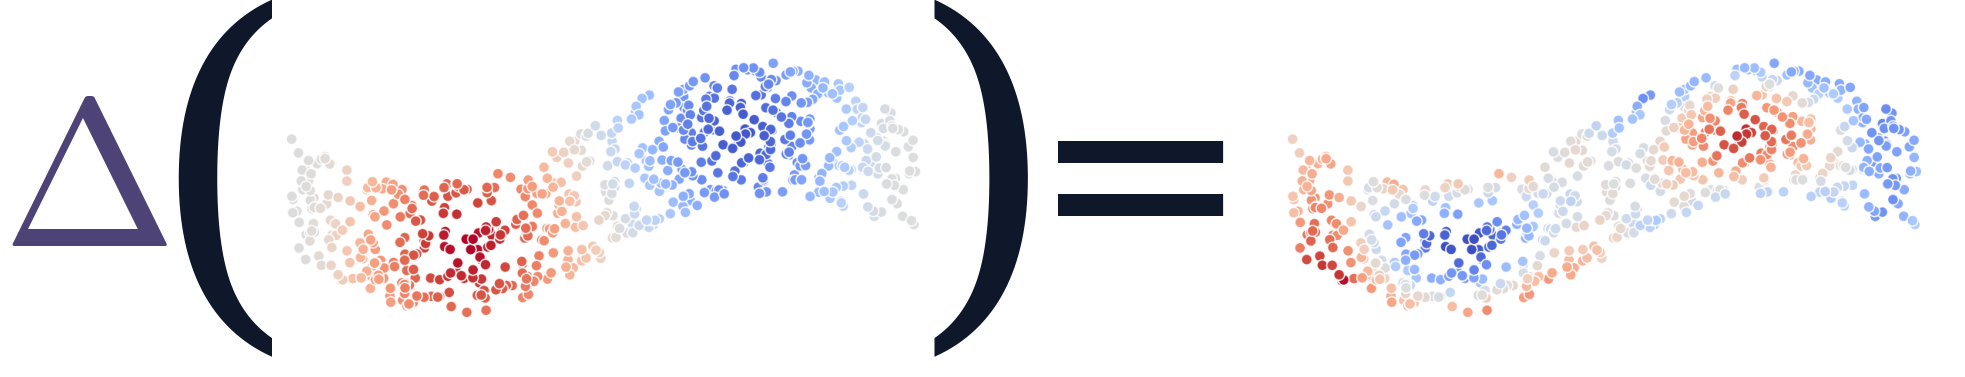
\includegraphics[width=0.98\linewidth]{figures/data_manifold_action.png}
    \vspace*{\fill}
  \end{minipage}\hfill
  \begin{minipage}[t][\toprowH][t]{0.48\linewidth}
    \centering
    {\small\textbf{Euclidean, 1D}\;\;
      $\Delta f = \dfrac{d^{2} f}{dx^{2}}$}\par
    \vspace{0.4ex}
    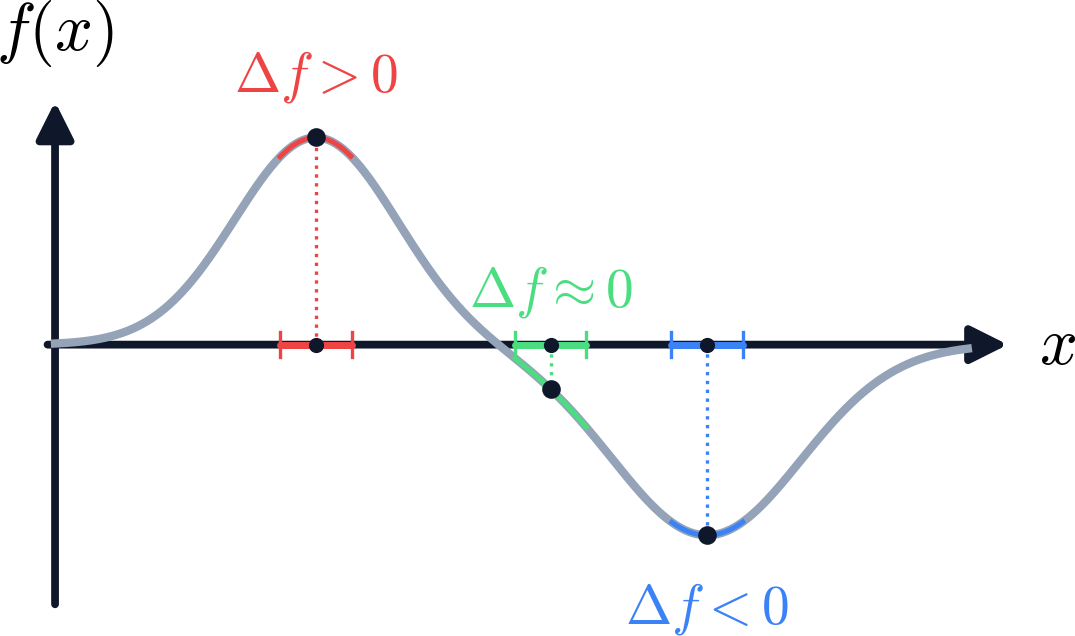
\includegraphics[width=0.95\linewidth]{figures/lap_euclidean_1d_stage_9.png}
  \end{minipage}
  \vspace{1.0ex}\par
  % Row 2
  \begin{minipage}[t]{0.48\linewidth}
    \centering
    {\small\textbf{Euclidean, 2D}\;\;
      $\Delta f = \partial_{u}^{2} f + \partial_{v}^{2} f$}\par
    \vspace{0.4ex}
    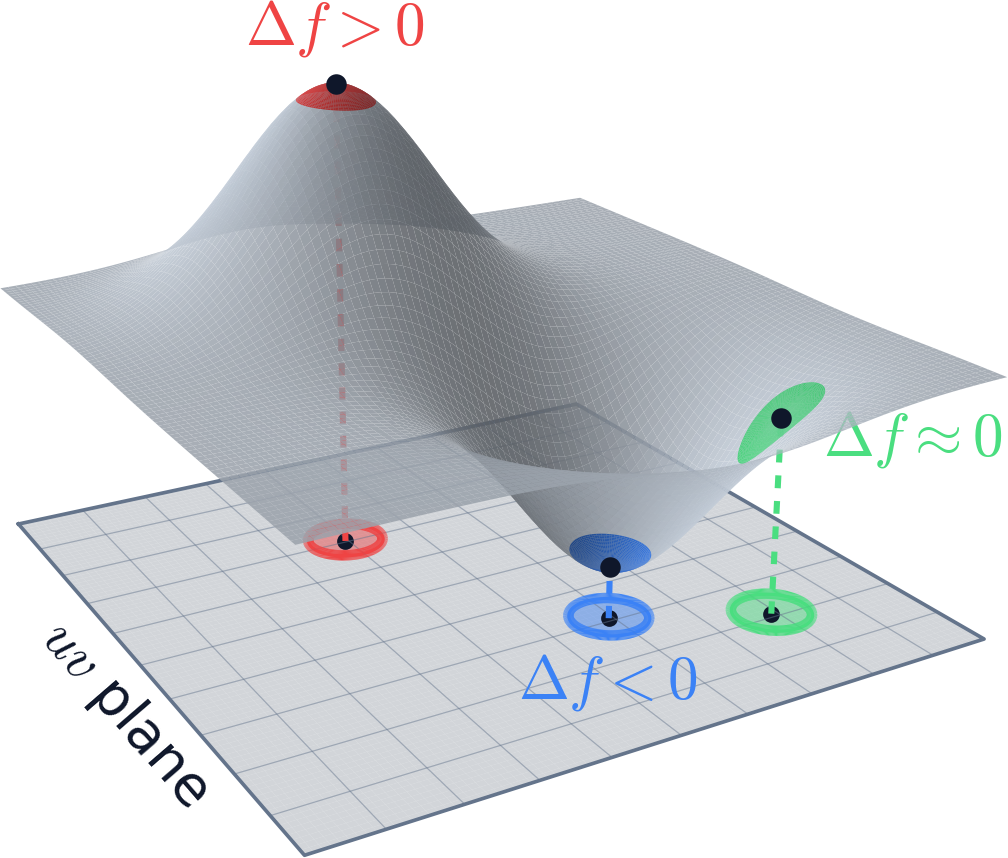
\includegraphics[width=0.95\linewidth]{figures/lap_euclidean_2d_stage_9.png}
  \end{minipage}\hfill
  \begin{minipage}[t]{0.48\linewidth}
    \centering
    {\small\textbf{Curved domain (LBO)}\;\;
      $\Delta_{\!\mathcal{M}} f = \operatorname{div}_{\!\mathcal{M}}\bigl(\nabla_{\!\mathcal{M}} f\bigr)$}\par
    \vspace{0.4ex}
    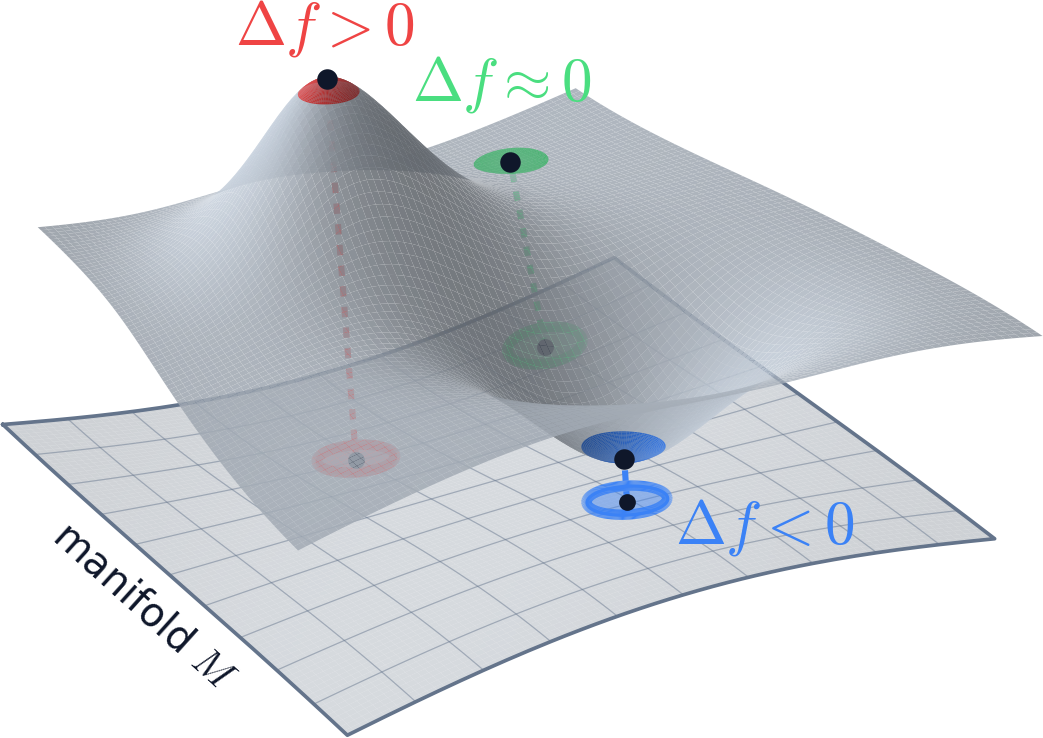
\includegraphics[width=0.95\linewidth]{figures/lap_curved_2d_stage_9.png}
  \end{minipage}
\end{block}

\begin{block}{A single spectral basis --- many families of tools}
  \centering\small
  % Freeze the cell width in absolute units NOW so it does NOT shrink to
  % a fraction of the inner minipage \linewidth when used inside the cell.
  \newlength{\appW}\setlength{\appW}{0.327\linewidth}%
  % 3 cells × 0.327 ≈ 0.98 of linewidth → ~2% left for two \hfill gaps.
  % Hard cap on image height — keeps tall-aspect tiles (Geodesics) from
  % dominating the row while leaving wide-aspect tiles unaffected.
  \def\appMaxH{8.5cm}%
  \def\appcell##1##2{%
    \begin{minipage}[b]{\appW}\centering
      \includegraphics[width=\appW, height=\appMaxH, keepaspectratio]{figures/##1}\par
      \vspace{0.25ex}\textbf{##2}
    \end{minipage}%
  }%
  \appcell{app_01_descriptors.png}{Shape descriptors}\hfill
  \appcell{app_02_corr_lion.png}{Shape correspondence}\hfill
  \appcell{app_03_manifold_learning.png}{Manifold learning}\par
  \vspace{0.6ex}
  \appcell{app_05_geometry_processing.png}{Geodesics}\hfill
  \appcell{app_07_mesh_smoothing.png}{Mesh smoothing}\hfill
  \appcell{app_09_arap_horse.png}{Shape deformation}\par
\end{block}

\begin{block}{Computing the Laplacian eigenstructure, the traditional way}
  \centering
  % Freeze the cell width in absolute units so it does not collapse to a
  % fraction of the inner cell linewidth.
  \newlength{\pipeColW}\setlength{\pipeColW}{0.245\linewidth}%
  \newlength{\pipeImgW}\setlength{\pipeImgW}{0.85\pipeColW}%
  \def\pipeImg##1{%
    \includegraphics[width=\pipeImgW, height=8.5cm, keepaspectratio]{figures/##1}%
  }%
  % Big math for the right two columns.
  \def\pipeEq##1{{\huge $##1$}}%
  \setlength{\tabcolsep}{4pt}\renewcommand{\arraystretch}{1.1}%
  \begin{tabular}{@{}
      >{\centering\arraybackslash}m{\pipeColW}|%
      >{\centering\arraybackslash}m{\pipeColW}|%
      >{\centering\arraybackslash}m{\pipeColW}|%
      >{\centering\arraybackslash}m{\pipeColW}@{}}
    \textbf{Neighborhood extraction} &
    \textbf{Operator extraction} &
    \textbf{Eigensolve} &
    \textbf{Eigenbasis} \\[0.6ex]
    \pipeImg{pipeline_triangulation.png} &
    \pipeImg{pipeline_voronoi_cot.png} &
    \pipeEq{S\,\boldsymbol{\phi} = \lambda\, M\,\boldsymbol{\phi}} &
    \pipeEq{\{\boldsymbol{\phi}_i\},\; \{\lambda_i\}} \\[5cm]
    \pipeImg{pipeline_knn_graph.png} &
    \pipeImg{pipeline_heat_weights.png} &
    \pipeEq{L\,\mathbf{y} = \lambda\, D\,\mathbf{y}} &
    \pipeEq{\{\mathbf{y}_i\},\; \{\lambda_i\}} \\
  \end{tabular}%
\end{block}

\end{column}

% ───────────── Column 2 ─────────────
\begin{column}{\colwidthA}

\begin{block}{Explicit, discrete, and not differentiable.}
  \centering
  \newlength{\btColW}\setlength{\btColW}{0.31\linewidth}%
  \setlength{\tabcolsep}{4pt}\renewcommand{\arraystretch}{1.0}%
  \begin{tabular}{@{}
      >{\centering\arraybackslash}m{\btColW}
      >{\centering\arraybackslash}m{\btColW}
      >{\centering\arraybackslash}m{\btColW}@{}}
    % Row 1: visuals — big Δ, triangulation, no-grad network.
    {\fontsize{180}{200}\selectfont $\Delta$} &
    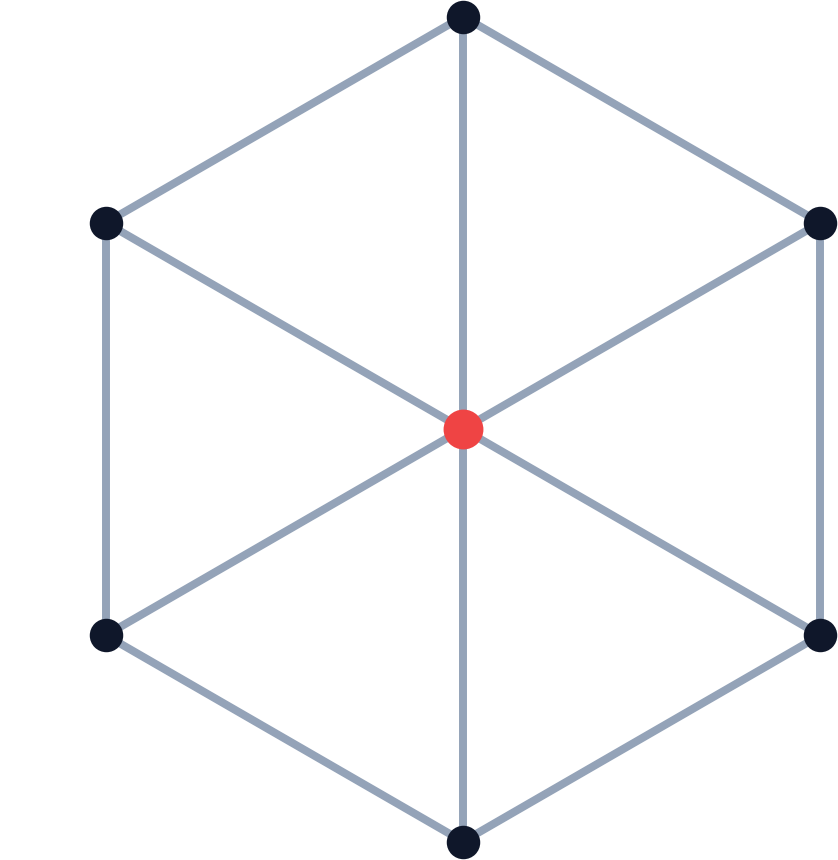
\includegraphics[width=0.82\btColW, height=11cm, keepaspectratio]{figures/pipeline_triangulation.png} &
    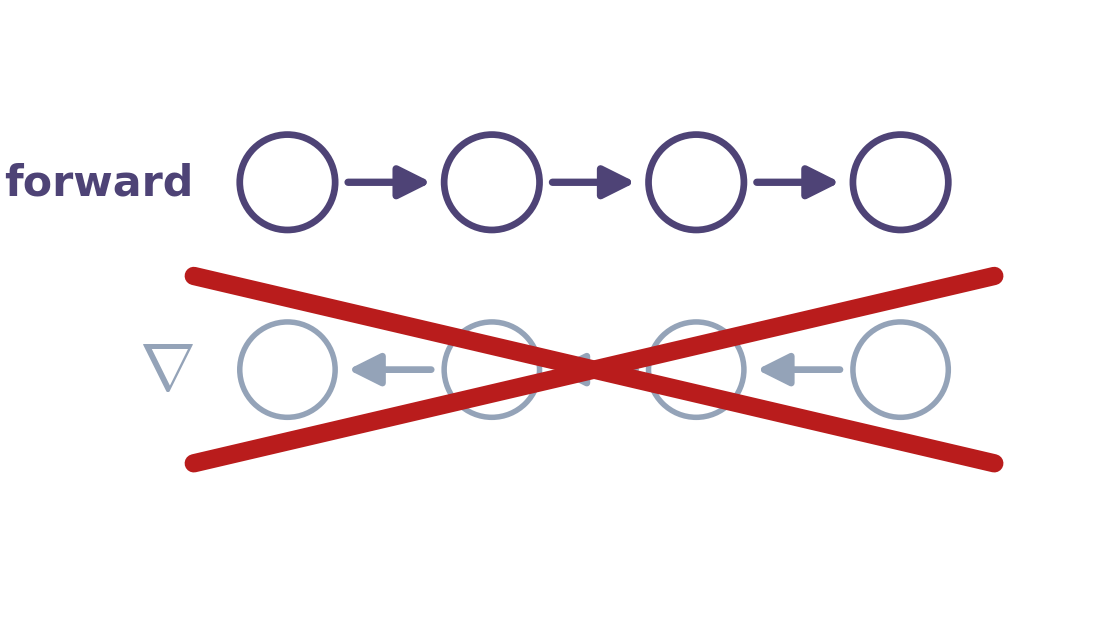
\includegraphics[width=0.95\btColW, height=11cm, keepaspectratio]{figures/bottleneck_no_grad.png} \\[1.0ex]
    % Row 2: original word struck out, replacement word in indigo.
    {\Large\textbf{\sout{explicit}}} &
    {\Large\textbf{\sout{discrete}}} &
    {\Large\textbf{\sout{not differentiable}}} \\[0.4ex]
    {\LARGE\textbf{\textcolor{cBrandFrom}{implicit}}} &
    {\LARGE\textbf{\textcolor{cBrandFrom}{continuous}}} &
    {\LARGE\textbf{\textcolor{cBrandFrom}{differentiable}}} \\
  \end{tabular}
\end{block}

\begin{block}{Skip the operator. Learn the eigenbasis directly.}
  \centering
  % Pill-shaped chips: an indigo background, white bold sans-ish text.
  \setlength{\fboxsep}{8pt}%
  \def\chip##1{\colorbox{cBrandFrom}{\color{white}\bfseries\large\strut\,##1\,}}%
  % Bypassed chip: dimmer fill + amber strikethrough through the text.
  \def\chipBy##1{\colorbox{cBrandFrom!45!white}{\color{white!85!black}\bfseries\large\strut\,{\color{cAccent}\sout{\textcolor{white!85!black}{##1}}}\,}}%
  \def\arr{\;\textcolor{cBrandTo}{\LARGE\,$\boldsymbol{\rangle}$\,}\;}%

  {\large\textbf{Traditional}}\par\vspace{1.0ex}
  \chip{Point cloud}\arr\chipBy{Neighborhood extraction}\arr\chipBy{Operator extraction}\arr\chipBy{Eigensolve}\arr\chip{Eigenbasis}\par
  \vspace{4ex}
  {\large\textbf{Ours}}\par\vspace{1.0ex}
  \chip{Point cloud}\arr\chip{\hspace{3em}Neural network\hspace{3em}}\arr\chip{Eigenbasis}\par
\end{block}

\begin{block}{The optimal $k$-term basis is the eigenbasis}
  \centering
  \begin{minipage}[t]{0.48\linewidth}
    \centering
    \textbf{Arbitrary basis}\par\vspace{0.4ex}
    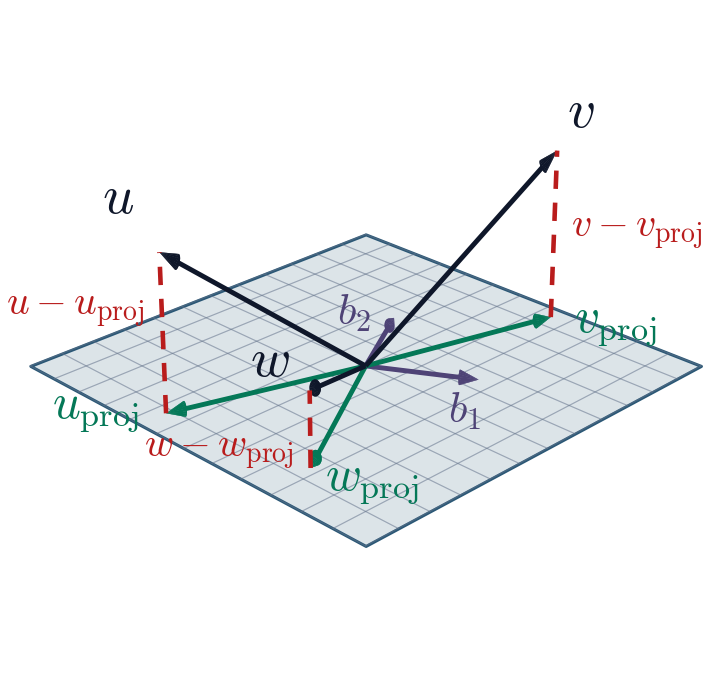
\includegraphics[width=0.95\linewidth]{figures/optimal_basis_step7.png}\par
    \vspace{0.3ex}
    {\footnotesize\itshape Large residual on every vector --- the basis ignores the data.}
  \end{minipage}\hfill
  \begin{minipage}[t]{0.48\linewidth}
    \centering
    \textbf{Optimal $k$-term basis}\par\vspace{0.4ex}
    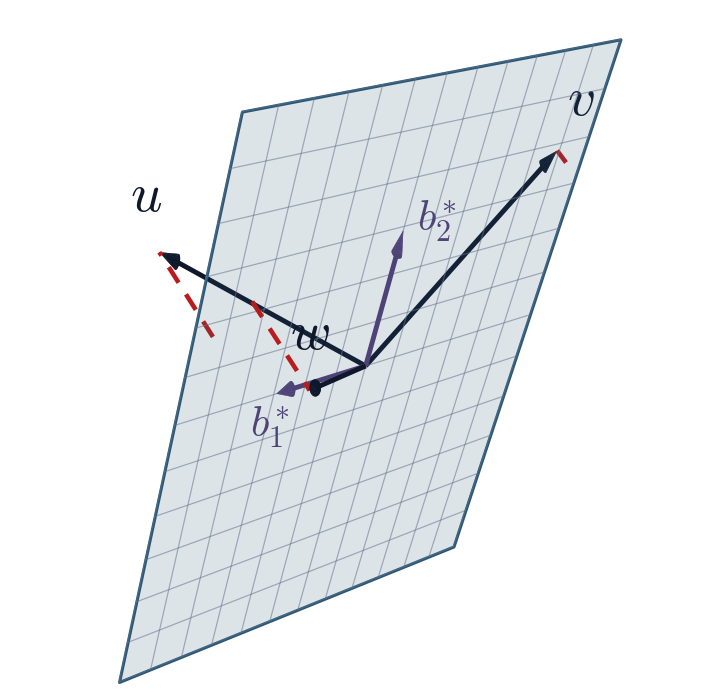
\includegraphics[width=0.95\linewidth]{figures/optimal_basis_step9.png}\par
    \vspace{0.3ex}
    {\footnotesize\itshape Residuals collapse --- $\{b_i^*\}$ are the top-$k$ eigenvectors of $\sum_j v_j v_j^\top$.}
  \end{minipage}
\end{block}

\begin{block}{On a curve or an image, this eigenbasis is the DCT}
  \centering
  \begin{minipage}[t]{0.48\linewidth}
    \centering
    \textbf{1D --- the curve $[0, L]$}\par\vspace{0.5ex}
    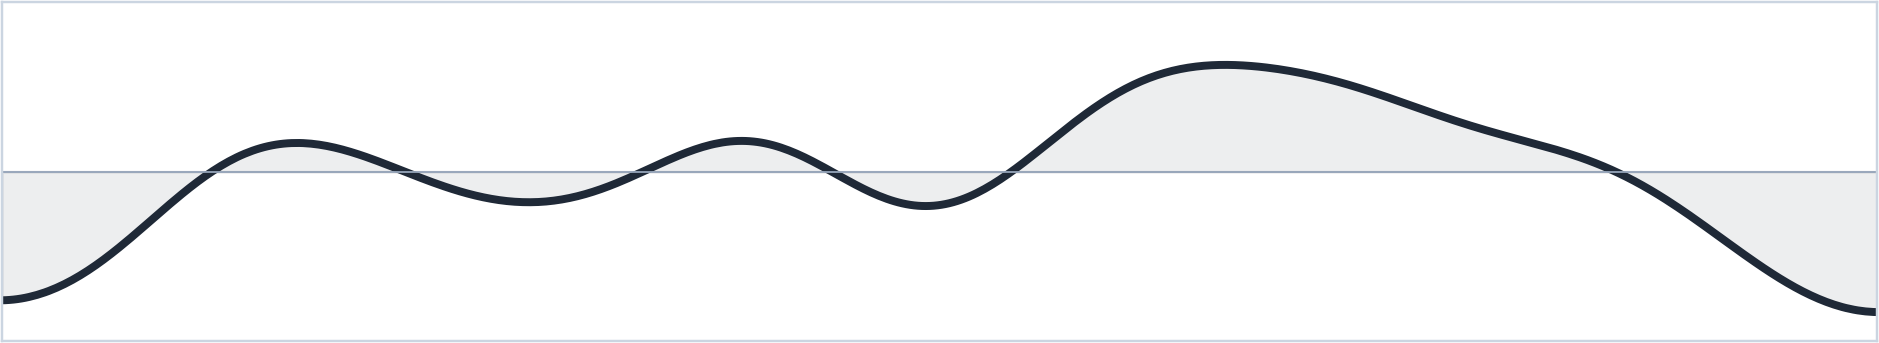
\includegraphics[width=0.92\linewidth, height=2.6cm, keepaspectratio]{figures/dct_1d_sample.png}\par
    \vspace{0.6ex}
    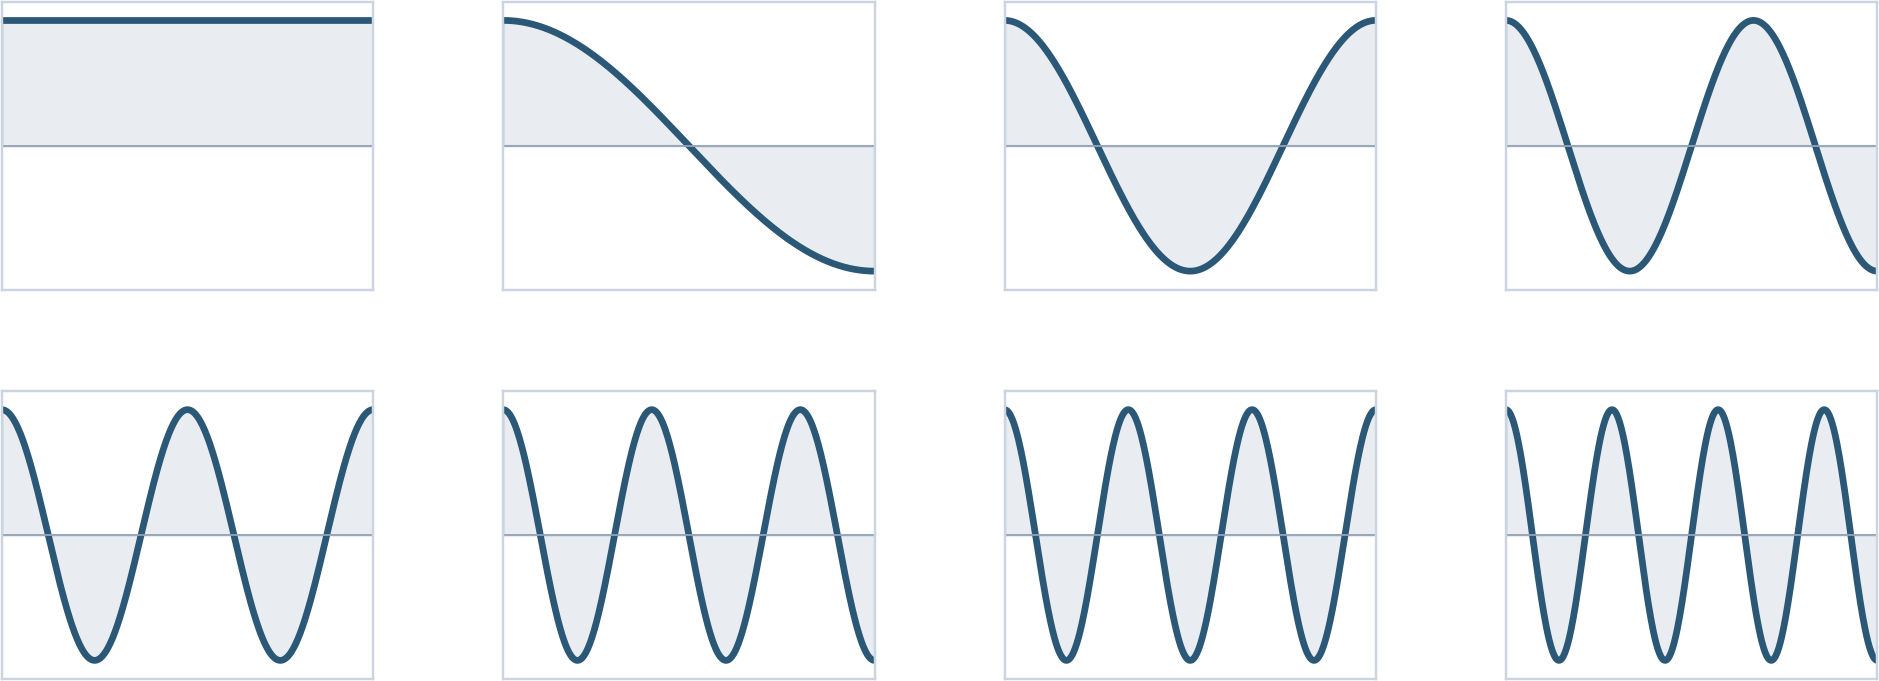
\includegraphics[width=0.92\linewidth, height=9cm, keepaspectratio]{figures/dct_1d_basis.png}\par
    \vspace{0.5ex}
    $\varphi_n(x) = \cos\!\left(\dfrac{n\pi x}{L}\right)$
  \end{minipage}\hfill
  \begin{minipage}[t]{0.48\linewidth}
    \centering
    \textbf{2D --- the image rectangle}\par\vspace{0.5ex}
    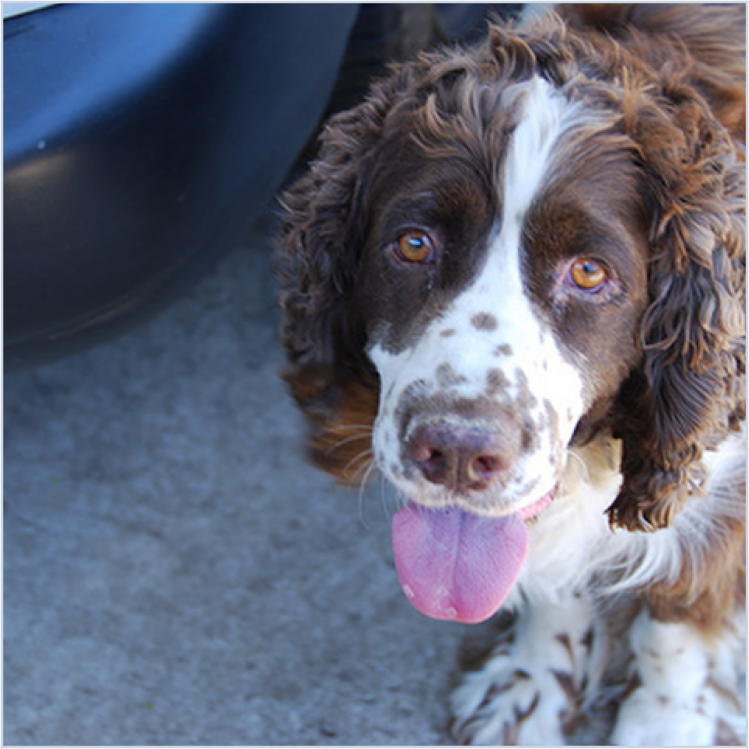
\includegraphics[width=0.92\linewidth, height=2.6cm, keepaspectratio]{figures/dct_2d_sample.png}\par
    \vspace{0.6ex}
    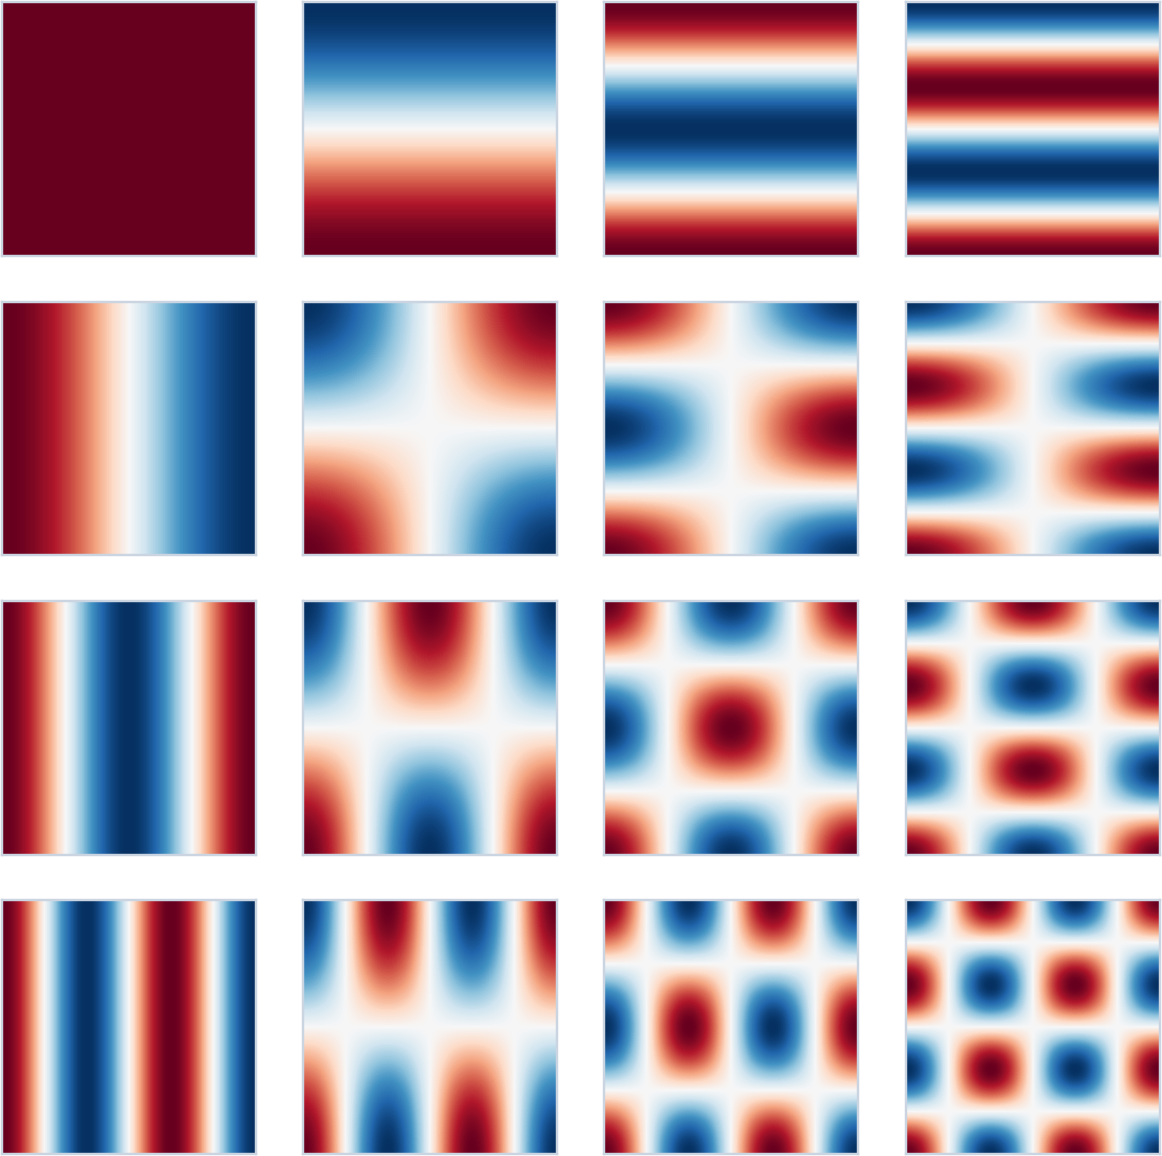
\includegraphics[width=0.92\linewidth, height=9cm, keepaspectratio]{figures/dct_2d_basis.png}\par
    \vspace{0.5ex}
    $\varphi_{n,m}(x, y) = \cos\!\left(\dfrac{n\pi x}{L_x}\right)\cos\!\left(\dfrac{m\pi y}{L_y}\right)$
  \end{minipage}\par
  \vspace{0.8ex}
  \centering\textbf{\large Euclidean Laplacian eigenbasis \;\textemdash\; Neumann boundary conditions.}
\end{block}

\begin{block}{The optimal $k$-term basis is the eigenbasis of $L$}
  \Large\justifying

  Let $L \succeq 0$ be the Laplacian and let
  \[
    \mathcal{C}_L \;=\; \bigl\{\, f \;:\; \langle f,\, L f\rangle \le 1 \,\bigr\},
    \qquad
    p_L \;=\; \mathrm{Uniform}(\mathcal{C}_L).
  \]

  \noindent\textbf{Theorem 1.}\;
  \emph{Among all orthonormal $k$-subspaces, the expected
        squared reconstruction error under $p_L$ is minimised by
        the first $k$ eigenvectors of $L$:}
  \[
    \arg\!\min_{\{b_i\}_{i=1}^{k}}\;
      \mathbb{E}_{f \sim p_L}\, \bigl\|f - \Pi_k f\bigr\|^{2}
    \;=\; \{\varphi_1, \dots, \varphi_k\}.
  \]

  \noindent\textbf{Theorem 2.}\;
  \emph{Under that basis the worst-case error is sharp:}
  \[
    \max_{f \in \mathcal{C}_L}\; \bigl\|f - \Pi_k f\bigr\|^{2}
    \;=\; \tfrac{1}{\lambda_{k+1}}.
  \]

  \vspace{0.4ex}
  \hfill {\small\itshape Aflalo, Brezis, Bruckstein, Kimmel \& Sochen,
                          C.\ R.\ Math.\ \textbf{354} (2016).}
\end{block}

\end{column}

% ───────────── Column 3 ─────────────
\begin{column}{\colwidthA}

\begin{block}{Best $k$-truncated basis on curved domains --- the Laplace--Beltrami eigenbasis}
  \centering

  % Thumbnail size (frozen as an absolute length so it doesn't shrink
  % inside the inner minipages — see the same trick used elsewhere).
  \newlength{\mbThumb}\setlength{\mbThumb}{0.13\linewidth}%
  \def\mbImg##1{\includegraphics[width=\mbThumb, height=\mbThumb, keepaspectratio]{figures/##1}}%
  \def\mbDots{\;\raisebox{0.5ex}{\Large$\cdots$}\;}%
  \def\mbCap##1{\par\vspace{0.3ex}{\small\textbf{##1}}\par}%

  % ── Row 1 — smooth manifold | sampled manifold | smooth scalar functions
  \begin{minipage}[t]{0.22\linewidth}\centering
    \mbImg{manifold_pc_mesh.png}\mbCap{smooth manifold}
  \end{minipage}\hfill
  \begin{minipage}[t]{0.22\linewidth}\centering
    \mbImg{manifold_pc_points.png}\mbCap{sampled manifold}
  \end{minipage}\hfill
  \begin{minipage}[t]{0.52\linewidth}\centering
    \mbImg{manifold_pc_signal_diff_01.png}\,
    \mbImg{manifold_pc_signal_diff_02.png}\mbDots
    \mbImg{manifold_pc_signal_diff_03.png}\,
    \mbImg{manifold_pc_signal_diff_04.png}
    \mbCap{smooth scalar functions}
  \end{minipage}\par
  \vspace{1.2ex}

  % ── Bases — four rows.
  \def\mbBasisRow##1{%
    \mbImg{manifold_pc_basis_##1_0.png}\,%
    \mbImg{manifold_pc_basis_##1_1.png}\,%
    \mbImg{manifold_pc_basis_##1_2.png}\mbDots
    \mbImg{manifold_pc_basis_##1_47.png}\,%
    \mbImg{manifold_pc_basis_##1_48.png}\,%
    \mbImg{manifold_pc_basis_##1_49.png}%
  }%

  \mbBasisRow{1}\mbCap{orthogonal basis \#1}\vspace{0.9ex}
  \mbBasisRow{2}\mbCap{orthogonal basis \#2}\vspace{0.9ex}

  % ── Highlighted LBO basis (the winner)
  {\setlength{\fboxsep}{6pt}%
   \fcolorbox{cBrandFrom}{cBgSoft}{%
     \begin{minipage}{0.95\linewidth}\centering
       \mbBasisRow{4}\mbCap{LBO eigenbasis \;---\; optimal $k$-truncated basis}
     \end{minipage}%
   }}
\end{block}

\begin{block}{Our pipeline}
  \centering
  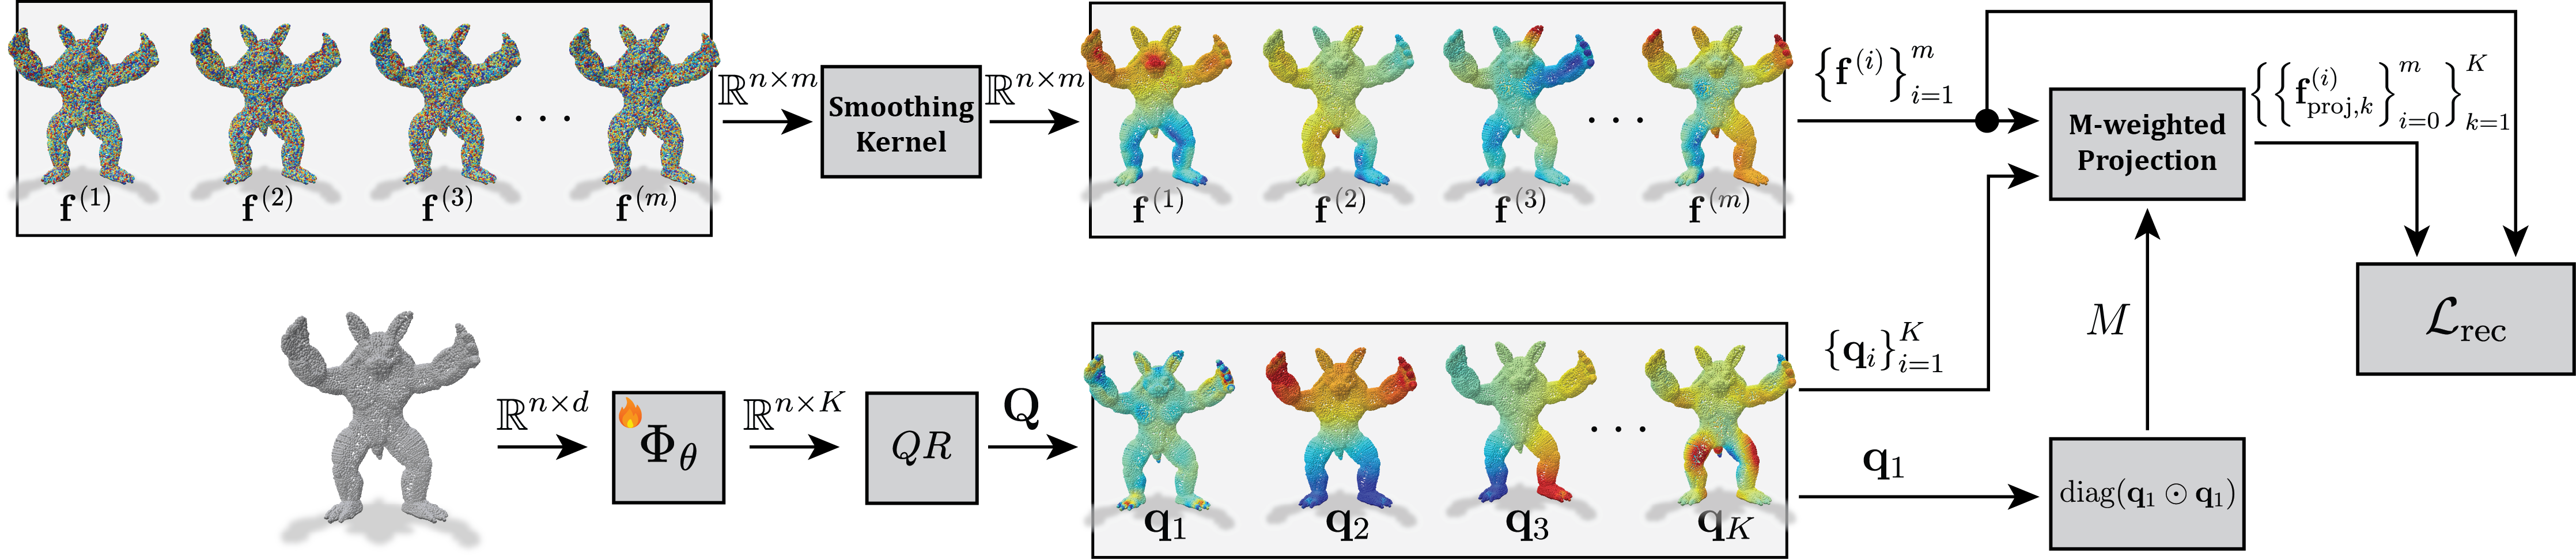
\includegraphics[width=\linewidth]{figures/pipeline.png}\par
  \vspace{1.0ex}

  \large
  Train end-to-end with the average reconstruction loss
  \[
    \mathcal{L}_{\text{rec}} \;=\;
    \frac{1}{m K}\;
    \sum_{i=1}^{m}\; \sum_{k=1}^{K}\;
    \bigl\lVert\, f^{(i)} \;-\; f^{(i)}_{\text{proj},\,k}\,\bigr\rVert_{2}^{2},
  \]
  measuring how well the first $k$ predicted basis vectors reconstruct
  each probe $f^{(i)}$, averaged over $i$ and $k$.
\end{block}

\end{column}

% ───────────── Column 4 ─────────────
\begin{column}{\colwidthA}

\begin{block}{Beyond the LBO}
  Because the method never builds the operator explicitly, swapping
  Laplacians is trivial: change only the probe sampler $p_L$.

  \vspace{0.3ex}
  \textbf{Hadamard probes.}\; Substituting random Hadamard probes
  recovers the same eigenbasis at any prefix.

  \vspace{0.3ex}
  \textbf{Schrödinger operator.}\; Adding a potential
  $V(x)$ to the probe energy yields the Schrödinger eigenstructure
  $\bigl(-\Delta + V\bigr)\phi_i = \lambda_i\,\phi_i$.

  \vspace{0.3ex}
  \centering
  \includegraphics[width=\linewidth]{figures/schrodinger_grid.pdf}
\end{block}

\begin{block}{Image manifold}
  The same recipe applied to CLIP / DINOv2 embeddings of Imagenette and
  STL10 recovers clusters and outperforms UMAP, t-SNE, PCA, and
  Laplacian eigenmaps on NMI \& ARI.
  \vspace{0.3ex}
  \centering
  \includegraphics[width=0.95\linewidth]{figures/nmi_ari_bars.pdf}
\end{block}

\begin{block}{Take-aways}
  \begin{itemize}
    \item One differentiable map replaces the entire traditional
          eigenstructure pipeline.
    \item Generalises across shapes, sampling resolutions, and
          operator families (LBO, Schrödinger, Hadamard).
    \item Trained on 3 K points, inferred on 12 K --- no degradation.
  \end{itemize}
\end{block}

\begin{block}{Acknowledgements \& code}
  We thank the CVPR area chair and reviewers for valuable feedback.
  Code, data, and the full paper:\par
  \textcolor{cBrandFrom}{\textbf{github.com/royvelich/learning-eigenstructures}}
\end{block}

\end{column}

\end{columns}
\end{frame}
\end{document}
